\documentclass[aspectratio=169]{beamer}
\usepackage[utf8]{inputenc}
\usepackage[english]{babel}
\usepackage[T1]{fontenc}
\usepackage[document]{ragged2e}
\usepackage{pgf-pie}
\usepackage{hyperref}
\usepackage{multicol}
\renewcommand{\sum}{170}

\usepackage{tikz}
% \usetikzlibrary{decorations.pathreplacing,positioning, arrows.meta}
\frenchspacing % Don't put two spaces after periods.
\usepackage{pgfpages}

\setbeameroption{hide notes}

\setbeamerfont{note date}{size=\scriptsize}
\setbeamerfont{note title}{size=\footnotesize}
\setbeamerfont{note page}{size=\footnotesize}

\usepackage{graphicx}
\usetheme{metropolis}

\begin{document}

% The metadata of the presentation
\title[Worlds]{Worlds}
\subtitle[]{A Distributed MMO}
\author[]{Ryan Walker\footnote{\texttt{ryan.cjw@gmail.com, \href{worldsmmo.com}{worldsmmo.com}}}}
\date{\today} % Replace with date of the presentation


\begin{frame}
  \maketitle
  \note{
    I'm the note from the title page.
  }
\end{frame}

\begin{frame}{Identity}
\[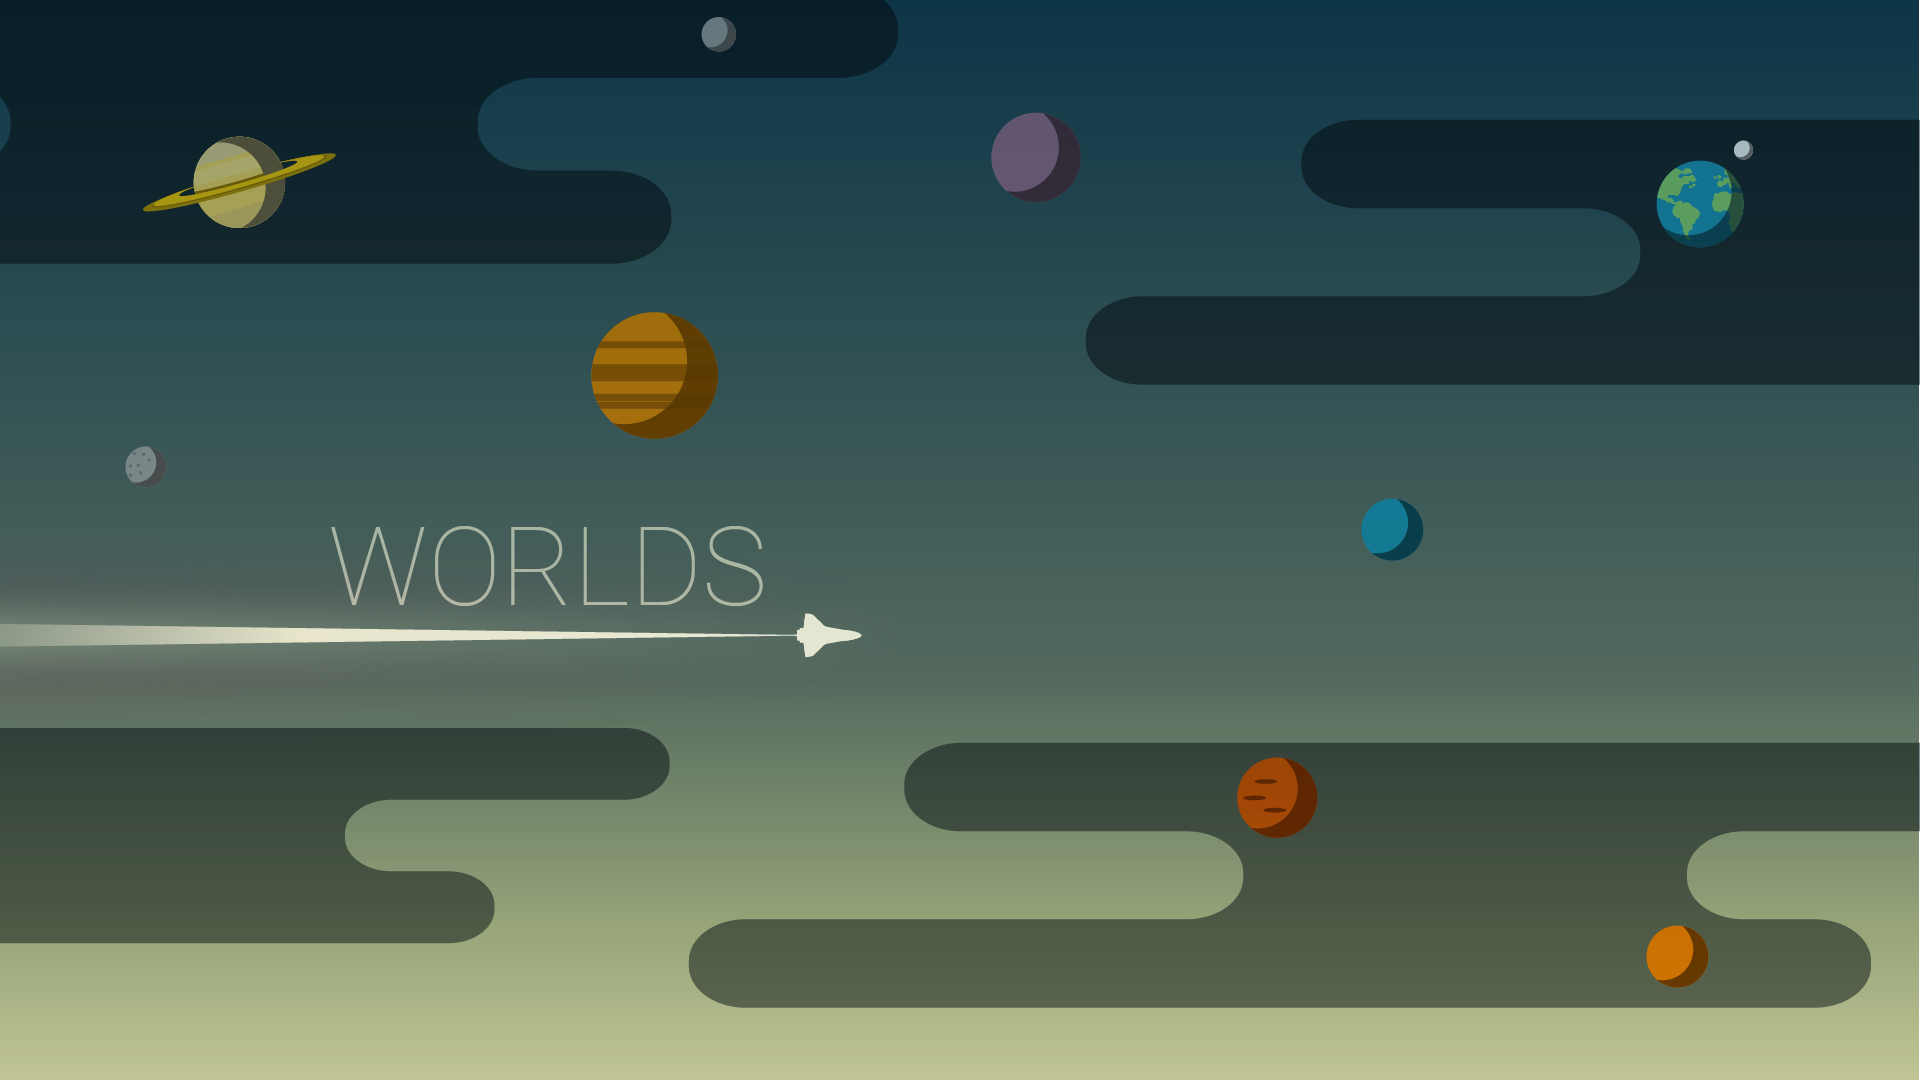
\includegraphics[scale=0.15, trim={0 4cm  0 4cm},clip]{Header.png}\] 
Worlds is the economic backbone for a distributed massively multiplayer online
game (MMO). Is enables players to move digital assets throughout multiple games,
built by independent developers, forming one congruent universe.  
\end{frame}


\begin{frame}{Mission}
Worlds will be the first open and scaleable infrastructure for building an
unbounded MMO. This platform will lead to the growth of the largest online game
ever created.
\end{frame}


\begin{frame}{Problem}
% The economy of an open world comes down to game theory. 
Allowing any user to modify the source code of a game enables them to create
unbounded resources; this creates an economic imbalance.  
\\~\\
Worlds implements a smart contract to manage the resources
ensuring that digital wealth cannot be created from nothing.
This is done by backing ingame assets against a token, WOR.
\end{frame}

\begin{frame}{Blockchain Infrastructure}
\end{frame}

\begin{frame}{Gaming Infrastructure}
\begin{columns}
\begin{column}{0.5\textwidth}
    \centering
    \textbf{Realm One}
    \\~\\
    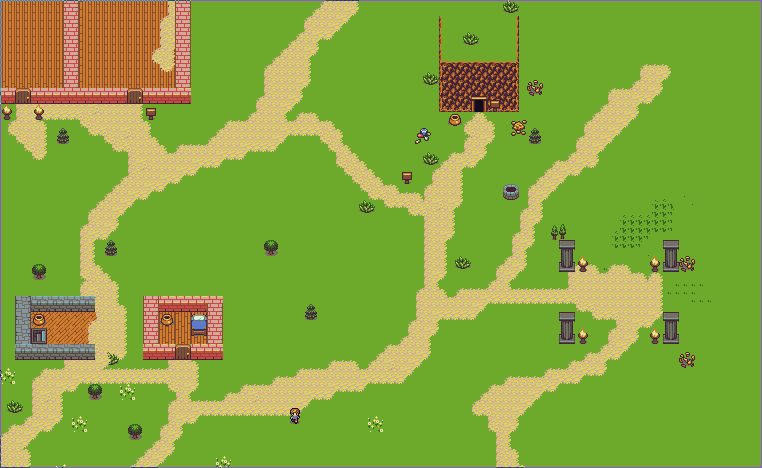
\includegraphics[scale=0.2]{realm.png}
    \justify
    Realm One is the first game that will be integrated into the Worlds
    ecosystem. It is developed by the Worlds team and is completely open
    source.

\end{column}
\begin{column}{0.5\textwidth}  %%<--- here
    \centering
    \textbf{Minecraft Fork}
    \\~\\
    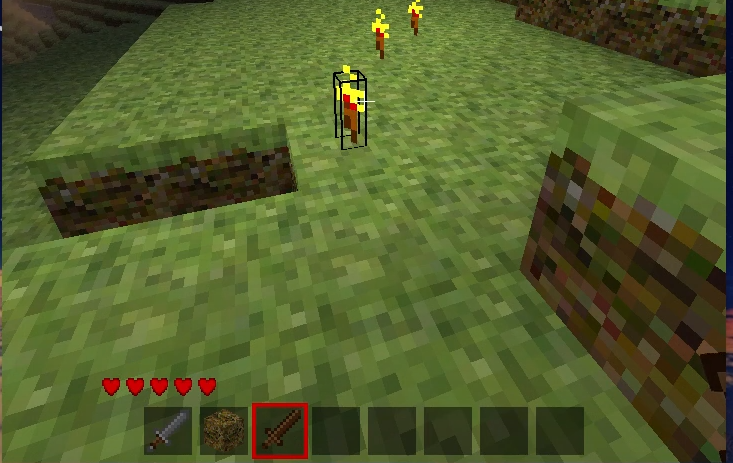
\includegraphics[scale=0.2]{minetest.png}
    \justify
    Realm One is the first game that will be integrated into the Worlds
    ecosystem. It is developed in the Rust programming language. 
\end{column}
\end{columns}
\end{frame}


\begin{frame}{Startup}
    To drive adoption we need to build an addicting game that will attract people
    from outside the blockchain community. This where the funding will be used for.
    \\~\\
    Existing game developers have no intensification to integrate with Worlds
    yet.  We need an open source platform that can be easily forked to build a
    world.
\end{frame}

\begin{frame}{Advantage}
    Existing projects, namely Enjin and Decentraland, are built using Ethereum. Which
    has not scaled yet and suffers from high gas cost. Worlds is built on EOSIO and will
    make a seperate chain that will be specific to Worlds.

    The projects above are trying to find developers to build into their ecosystem, however
    it's almost impossible to convince them to open source their games. A completely open
    source initial game is integral to scaling the network.
\end{frame}

\begin{frame}{Advantage}
    Traditionally there is no economic incentive to build an open source game. With worlds
    this is not the case, the token distribution is such that a game is successful and people
    and there are forks, players and developers will still be required to purchase game tokens.
    \\~\\
    As the demand for tokens increases, so will the price, makeing the tokenholders their ROI.
\end{frame}

\begin{frame}{Roadmap}
\begin{center}
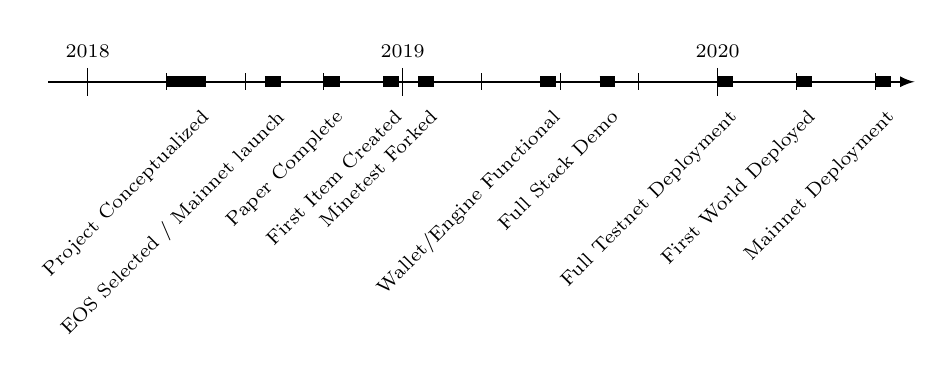
\begin{tikzpicture}
\draw[thick, -latex] (-0.5,0) -- (10.5,0);
%big ticks
\foreach \x in {0,4,8}
\draw (\x cm,5pt) -- (\x cm,-5pt);
%little ticks
\foreach \x in {1,2,3,5,6,7,9,10}
\draw (\x cm,3pt) -- (\x cm,-3pt);
%yr labels
\foreach \x/\descr in {0/2018,4/2019,8/2020}
\node[font=\scriptsize, text height=1.75ex,
text depth=.5ex] at (\x,0.4) {$\descr$};
%events

\draw[line width=4pt] (1,0) -- +(0.5,0)node[below left=2pt ,rotate=45]{\scriptsize Project Conceptualized};
\draw[line width=4pt] (2.25,0) -- +(0.2,0)node[below left=2pt ,rotate=45]{\scriptsize EOS Selected / Mainnet launch};
\draw[line width=4pt] (3,0) -- +(0.2,0)node[below left=2pt ,rotate=45]{\scriptsize Paper Complete};
\draw[line width=4pt] (3.75,0) -- +(0.2,0)node[below left=2pt ,rotate=45]{\scriptsize First Item Created};
\draw[line width=4pt] (4.2,0) -- +(0.2,0)node[below left=2pt ,rotate=45]{\scriptsize Minetest Forked};
\draw[line width=4pt] (5.75,0) -- +(0.2,0)node[below left=2pt ,rotate=45]{\scriptsize Wallet/Engine Functional};
\draw[line width=4pt] (6.5,0) -- +(0.2,0)node[below left=2pt ,rotate=45]{\scriptsize Full Stack Demo};
\draw[line width=4pt] (8,0) -- +(0.2,0)node[below left=2pt ,rotate=45]{\scriptsize Full Testnet Deployment};
\draw[line width=4pt] (9,0) -- +(0.2,0)node[below left=2pt ,rotate=45]{\scriptsize First World Deployed};
\draw[line width=4pt] (10,0) -- +(0.2,0)node[below left=2pt ,rotate=45]{\scriptsize Mainnet Deployment};

\end{tikzpicture}
\end{center}
\end{frame}

\begin{frame}{Token Cap Table}

\begin{figure}[H]
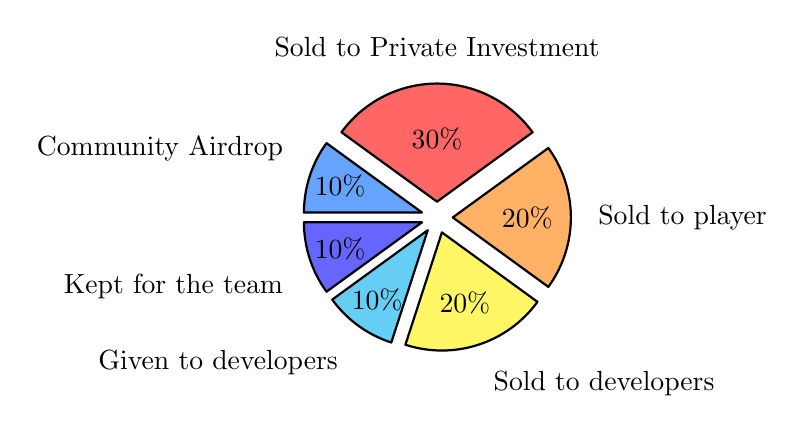
\begin{tikzpicture}

\pie [rotate = 180, radius=1.5, explode=0.2]
{
 10/Kept for the team,
 10/Given to developers, 
 20/Sold to developers, 
 20/Sold to player, 
 30/Sold to Private Investment,
 10/Community Airdrop
}

\end{tikzpicture}
\end{figure}

\end{frame}

\end{document}

\begin{frame}{Fundraising}

\begin{figure}[H]
Fundraising target for year one: \textbf{\$\sum k}
\begin{center}
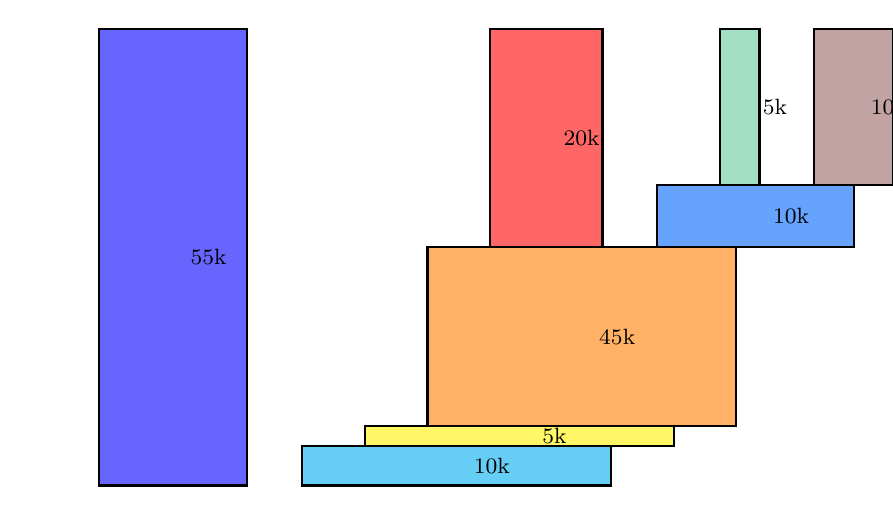
\begin{tikzpicture}
\footnotesize
\pie [square, radius=2.9, text=legend, after number = {k}, sum=\sum]
{55/Personal Wage,
 10/Office Space, 
 5/Graphic Design,
 45/Contract Game Developers,
 20/UI and UX ,
 10/Concept Art,
 5/Web Development,
 10/Server Fees,
 10/Security Audits
}
\end{tikzpicture}
\label{funding}
\end{center}
\end{figure}
\end{frame}

\begin{frame}{Fundraising}
The existing development has been done on my free time. I am looking to raise seed funding to make this my full time job. I am offering 5\% of the total supply WOR for \$\sum k. Following the mainnet launch, I will be raising a series A.
\end{frame}

\begin{frame}{Thank You}
I appreciate your consideration. Please reach out with any questions or feedback!
\\ \vfill
\begin{minipage}{0.5\textwidth}
\[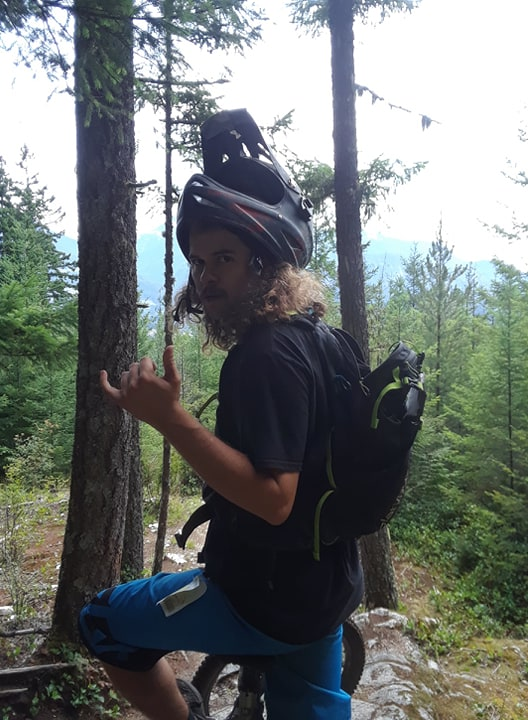
\includegraphics[scale=0.25, trim={0 2cm  0 2cm},clip]{me.jpg}\] 
\end{minipage}%
\begin{minipage}{0.5\textwidth}
Ryan Walker \\ Ryan.cjw@gmail.com \\  
\\~\\
\href{worldsmmo.com}{worldsmmo.com} \\ \href{https://www.youtube.com/watch?v=OrOZVr-j92A}{Demo}
\end{minipage}
\end{frame}

\end{document}
